% Created 2024-03-14 Thu 13:15
% Intended LaTeX compiler: pdflatex
\documentclass[presentation]{beamer}
\usepackage[utf8]{inputenc}
\usepackage[T1]{fontenc}
\usepackage{graphicx}
\usepackage{longtable}
\usepackage{wrapfig}
\usepackage{rotating}
\usepackage[normalem]{ulem}
\usepackage{amsmath}
\usepackage{amssymb}
\usepackage{capt-of}
\usepackage{hyperref}
\mode<beamer>{\usetheme{Madrid}}
\definecolor{SUred}{rgb}{0.59375, 0, 0.17969} % SU red (primary)
\definecolor{SUblue}{rgb}{0, 0.17578, 0.38281} % SU blue (secondary)
\setbeamercolor{palette primary}{bg=SUred,fg=white}
\setbeamercolor{palette secondary}{bg=SUblue,fg=white}
\setbeamercolor{palette tertiary}{bg=SUblue,fg=white}
\setbeamercolor{palette quaternary}{bg=SUblue,fg=white}
\setbeamercolor{structure}{fg=SUblue} % itemize, enumerate, etc
\setbeamercolor{section in toc}{fg=SUblue} % TOC sections
% Override palette coloring with secondary
\setbeamercolor{subsection in head/foot}{bg=SUblue,fg=white}
\setbeamercolor{date in head/foot}{bg=SUblue,fg=white}
\institute[SU]{Shenandoah University}
\titlegraphic{\includegraphics[width=0.5\textwidth]{\string~/Documents/suLogo/suLogo.pdf}}
\newcommand{\R}{\mathbb{R}}
\usepackage{tikz}
\usetheme{default}
\author{Chase Mathison\thanks{cmathiso@su.edu}}
\date{18 March 2024}
\title{Arc Length}
\hypersetup{
 pdfauthor={Chase Mathison},
 pdftitle={Arc Length},
 pdfkeywords={},
 pdfsubject={},
 pdfcreator={Emacs 29.1 (Org mode 9.6.7)}, 
 pdflang={English}}
\begin{document}

\maketitle

\section{Announcements}
\label{sec:org5b5e7e6}
\begin{frame}[label={sec:orgd07076d}]{Announcements}
\begin{enumerate}
\item Exam next week!
\item Office hours, 10am - 11am.
\end{enumerate}
\end{frame}

\section{Arc length}
\label{sec:orgaea960f}
\begin{frame}[label={sec:org9c3ff67}]{Arc length}
Now we're going to switch back to talking about applications of integration.  First up: arc length.

It's easy to calculate the length of a straight line.  
For instance, what is the length of the line segment given below?

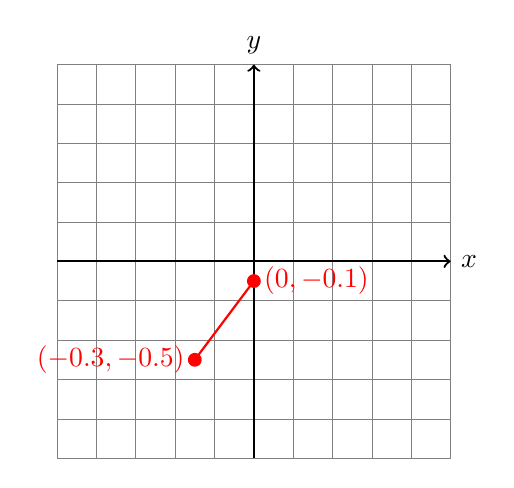
\begin{tikzpicture}[scale=2.5]
\draw[help lines,step=0.2] (-1,-1) grid (1,1);
\draw[thick,->] (-1,0) -- (1,0) node[below,right] {\(x \)};
\draw[thick,->] (0,-1) -- (0,1) node[above] {\(y \)};
\draw[thick,color=red] (-0.3,-0.5) node[below,left] {$(-0.3,-0.5)$} -- +(.3,.4) node[right] {$(0,-0.1)$};
\fill[red] (-0.3,-0.5) circle (1pt);
\fill[red] (0,-0.1) circle (1pt);
\end{tikzpicture}
\end{frame}

\begin{frame}[label={sec:org7edab61}]{Arc length}
Now, how could we try to calculate the length of the following curve
\(y = f(x)\)?

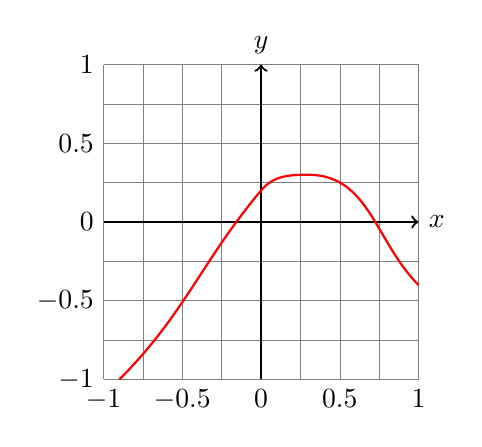
\begin{tikzpicture}[scale=2.0]
\draw[help lines, step=0.25] (-1,-1) grid (1,1);
\draw[thick,->] (-1,0) -- (1,0) node[right] {\(x\)};
\draw[thick,->] (0,-1) -- (0,1) node[above] {\(y \)};
\draw[thick,color=red] (-0.9,-1) to [out=45,in=-130] (0,0.2) to [out=50,in=180] (0.3,0.3) to [out=0,in=135] (1,-0.4);
\foreach \x in {-1,-0.5,...,1}
  \node[below] at (\x,-1) {$\x$};
\foreach \y in {-1,-0.5,...,1}
  \node[left] at (-1,\y) {$\y$};
\end{tikzpicture}

We don't know how this curve is defined, but we can try to approximate
the length using some straight lines, which are easy to calculate the
length of.
\end{frame}

\begin{frame}[label={sec:org67d2f2c}]{Arc length}
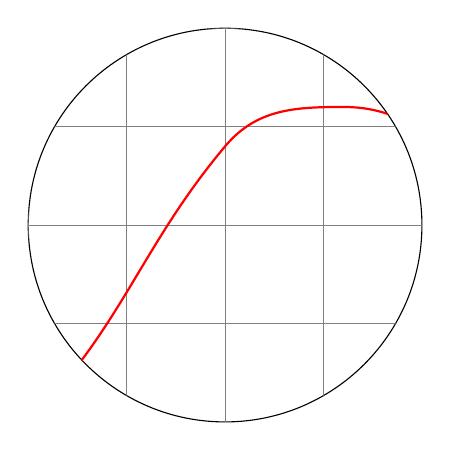
\begin{tikzpicture}[scale=5]
\draw[clip] (0,0) circle (0.5cm);
\draw[help lines, step=0.25] (-1,-1) grid (1,1);
\draw[thick,color=red] (-0.5,-0.5) to [out=45,in=-130] (0,0.2) to [out=50,in=180] (0.3,0.3) to [out=0,in=135] (0.9,-0.4);
\end{tikzpicture}
\end{frame}

\begin{frame}[label={sec:orgdf1e8a0}]{Arc length}
\end{frame}

\begin{frame}[label={sec:org60e2fd7}]{Arc length}
All of this has shown the following:
\begin{theorem}[Arc length of the graph of a smooth function]
Let \(f \left( x \right)\) be a differentiable function such that
\(f' \left( x \right)\) is continuous (i.e. \(f\) is \emph{smooth}) over
the interval \(\left[ a,b \right].\) The arc length of the portion of
the graph of \(y = f \left( x \right)\) between the points \(\left( a,f
\left( a \right) \right)\) and \(\left( b,f \left( b \right) \right)\) is given by
\[
s = \int\limits_a^b \sqrt{1 + \left[ f' \left( x \right) \right]^2}\,dx. \]
\end{theorem}

A word of warning:  many of the integrals that result from this
theorem are very difficult (though not impossible) to evaluate.  Some
of the methods that we've developed over the last several weeks will
help, but we'll still need to use technology for a lot of the
resulting integrals.
\end{frame}
\begin{frame}[label={sec:org5303f0c}]{Example}
What is the length of the curve defined by the function \(y = 2x^{3/2}\) on the interval \(\left[ 1,4 \right]?\)

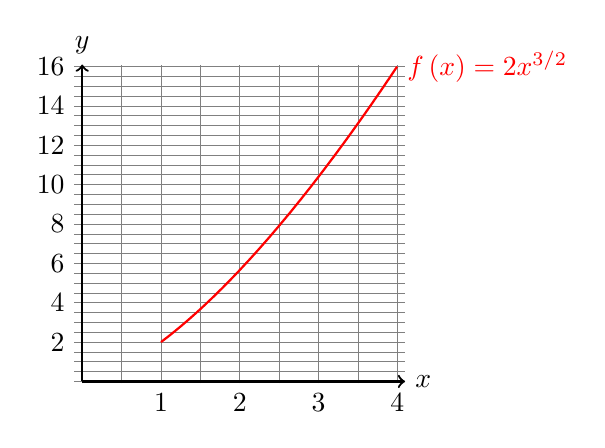
\begin{tikzpicture}[domain=1:2,xscale=1,yscale=0.25]
\draw[help lines,step=0.5cm] (-0.1,-0.1) grid (4.1,16.1);
\draw[thick,->] (0,0) -- (4.1,0) node[right] {\(x \)};
\draw[thick,->] (0,0) -- (0,16.1) node[above] {\(y \)};

\draw[color=red,thick] plot ({\x*\x},{2*\x*\x*\x}) node[right] {\(f \left( x \right) = 2x^{3/2} \)};
\foreach \x in {1,2,3,4}
  \node[below] at (\x,-0.1) {\(\x \)};
\foreach \y in {2,4,...,16}
  \node[left] at (-0.1,\y) {\(\y \)};
\end{tikzpicture}
\vspace{10in}
\end{frame}

\begin{frame}[label={sec:org6886b56}]{Example}
\end{frame}

\begin{frame}[label={sec:org931533b}]{Example}
What is the length of the parabola defined by \(y=x^2\) on the
interval \(\left[ 0,2 \right]\)?
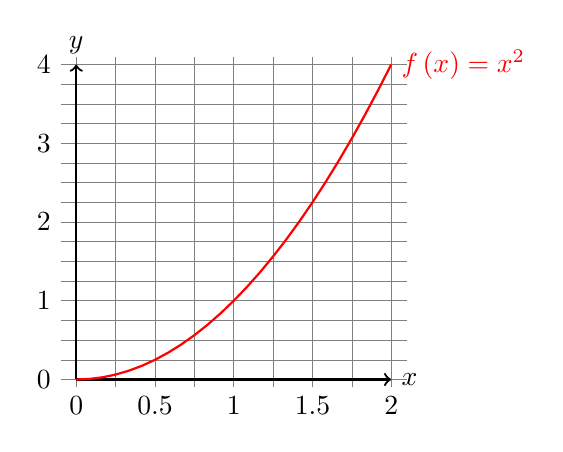
\begin{tikzpicture}[domain=0:2,xscale=2,yscale=1]
\draw[help lines,step=0.25cm] (-0.1,-0.1) grid (2.1,4.1);
\draw[thick,->] (0,0) -- (2,0) node[right] {\(x \)};
\draw[thick,->] (0,0) -- (0,4) node[above] {\(y \)};
\draw[color=red,thick] plot (\x,{\x*\x}) node[right] {\(f \left( x \right) = x^2 \)};
\foreach \x in {0,0.5,...,2}
  \node[below] at (\x,-0.1) {\(\x \)};
\foreach \y in {0,1,...,4}
  \node[left] at (-0.1,\y) {\(\y \)};
\end{tikzpicture}
\vspace{10in}
\end{frame}

\begin{frame}[label={sec:org4756aea}]{Example}
\end{frame}

\begin{frame}[label={sec:org5a2b135}]{Example}
Calculate the length of the curve defined by the function
\[
f \left( x \right) = \frac{x^4}{4} + \frac{1}{8x^2} \]
over the interval \(\left[ 1,2 \right]\).

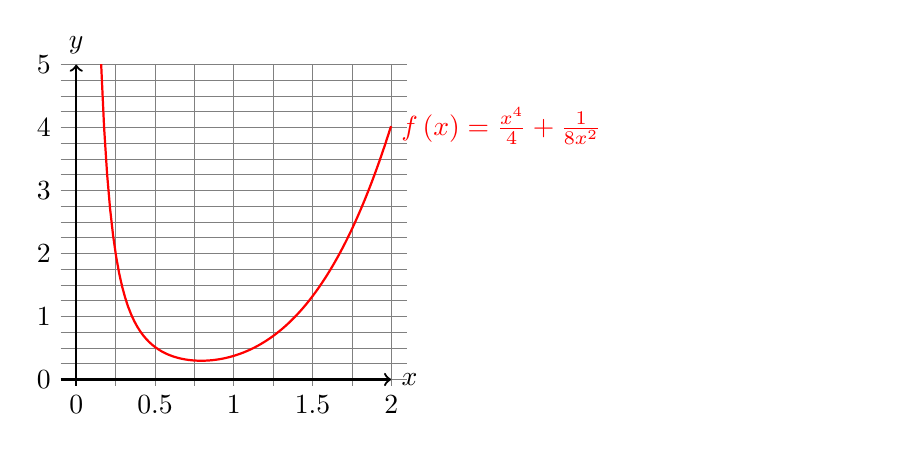
\begin{tikzpicture}[domain=0.1:2,samples=100,yscale=0.8,xscale=2]
\draw[help lines,step = 0.25] (-0.1,-0.1) grid (2.1,5);
\draw[->,thick] (-0.1,0) -- (2,0) node[right] {\(x \)};
\draw[->,thick] (0,-0.1) -- (0,5) node[above] {\(y \)};
\foreach \x in {0,0.5,...,2}
  \node[below] at (\x,-0.1) {\(\x \)};
\foreach \y in {0,1,...,5}
  \node[left] at (-0.1,\y) {\(\y \)};
\clip (-0.1,-0.1) rectangle (5.1,5);
\draw[thick,color=red] plot (\x,{0.25*pow(\x,4)+0.125*pow(\x,-2)}) node[right] {\(f \left( x \right) = \frac{x^4}{4} + \frac{1}{8x^2} \)};
\end{tikzpicture}
\vspace{10in}
\end{frame}

\begin{frame}[label={sec:org000af3c}]{Example}
\end{frame}

\begin{frame}[label={sec:org9bc9fb4}]{Arc length for functions of \(y\)}
If we want to find the arc length of some smooth function of \(y\),
say \(x = g \left( y \right),\) the formula is almost identical:
\begin{theorem}[Arc length (function of \(y\))]
Suppose \(x = g \left( y \right)\) is a smooth function of \(y\) on
the interval \(\left[ c,d \right].\)  Then the length of the curved
defined by \(x = g \left( y \right)\) is given by
\[
s = \int\limits_c^d \sqrt{1 + \left( g' \left( y \right)
\right)^2}\,dy. \]
\end{theorem}
\end{frame}

\begin{frame}[label={sec:org607400e}]{Example}
Find the arc length of the curve defined by
\[
x = \frac{e^y+e^{-y}}{2} \]
for \(y\) on the interval \(\left[ 0,1 \right].\)


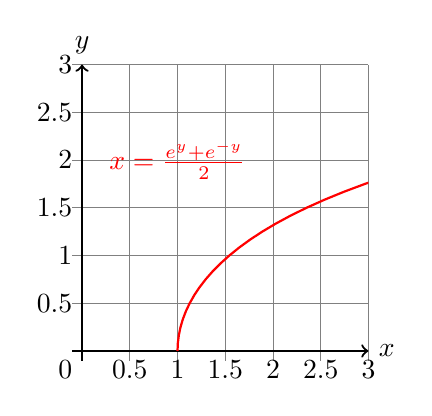
\begin{tikzpicture}[domain=0:2,scale=0.3\textwidth/3cm]
\draw[help lines,step=0.5] (-0.1,-0.1) grid (3,3);
\draw[thick,->] (-0.1,0) -- (3,0) node[right] {\(x \)};
\draw[thick,->] (0,-0.1) -- (0,3) node[above] {\(y \)};
\node[anchor = north east] at (0,0) {\(0 \)};
\foreach \x in {0.5,1,...,3}
  \node[below] at (\x,0) {\(\x \)};
\foreach \y in {0.5,1,...,3}
  \node[left] at (0,\y) {\(\y \)};
\clip (-0.1,-0.1) rectangle (3,3);
\draw[thick,color=red] plot ({0.5*(exp(\x)+exp(-\x))},\x) ;
\node[color=red] at (1,2) {\(x = \frac{e^y+e^{-y}}{2} \)};
\end{tikzpicture}
\vspace{10in}
\end{frame}

\begin{frame}[label={sec:orgf9113ba}]{Example}
\end{frame}
\end{document}